%% Elsevier 'elsarticle' template — Structures (review mode)
\pdfminorversion=7 % allow inclusion of up to PDF 1.7 graphics
\documentclass[review,12pt]{elsarticle} % ilk gönderimde review + tek sütun
\journal{Structures}
\biboptions{square}

%% Packages
\usepackage[english]{babel}
\usepackage{amsmath,amssymb,mathtools}
\usepackage{graphicx}
\usepackage{siunitx}
\usepackage{microtype}
\makeatletter
\AtBeginDocument{\@ifundefined{MT@orig@showhyphens}{}{\let\showhyphens\MT@orig@showhyphens}}
\makeatother
\usepackage{lineno}
\usepackage{booktabs}
\usepackage{tabularx}
\usepackage{array}
\usepackage{ragged2e} % daha iyi satır sonu için (opsiyonel)
\usepackage{placeins}



%% siunitx
\sisetup{
mode = match,
propagate-math-font = true,
reset-math-version = false,
reset-text-family = false,
reset-text-series = false,
reset-text-shape = false,
text-family-to-math = true,
text-series-to-math = true,
per-mode = symbol,
range-units = single,
range-phrase = --,
exponent-product = \times
}

%% Microtype
\microtypesetup{expansion,protrusion}
\emergencystretch=3em
\allowdisplaybreaks[1]

% --- HYPERREF EN SONDA ---
\usepackage{hyperref}
\makeatletter
\pdfstringdefDisableCommands{%% disable front-matter commands in PDF strings
\def\corref#1{}
\def\cortext#1{}
\def\cnotenum#1{}
\def\@corref#1{}
}
\makeatother
\newcolumntype{L}{>{\RaggedRight\arraybackslash}X}
\providecommand*{\theHpage}{\thepage}

\DeclareUnicodeCharacter{03B2}{\ensuremath{\beta}}
\begin{document}
\pagenumbering{roman}
\renewcommand*{\theHpage}{FR\roman{page}}
\begin{frontmatter}

\title{Hydro--thermal high-fidelity modelling and multi-objective design of fluid viscous dampers}

%% Authors
\author[aff1]{Ad Soyad\corref{cor1}}
\ead{email@kurum.edu.tr}
\cortext[cor1]{Corresponding author.}

\address[aff1]{Bölüm, Kurum, Şehir, Posta Kodu, Türkiye}

%% Abstract
\begin{abstract}
% 150–250 kelime: Amaç; hidrolik–termal FVD modeli (Cd(Re), kavitasyon, μ(T));
% 10-DOF yapısal model ve zaman entegrasyonu; çok-amaçlı GA (⟨IDR⟩, ⟨PFA⟩);
% başlıca bulgular (yüzdesel azaltımlar, güvenlik metrikleri); pratik tasarım ilkeleri.
\end{abstract}

%% Graphical abstract (ayrı PDF/PNG ekleyebilirsin)
\begin{graphicalabstract}
% \includegraphics[width=\linewidth]{figs/graphical_abstract.pdf}
\end{graphicalabstract}

%% Highlights (3–5 madde)
\begin{highlights}
\item Physics-informed fluid viscous damper with Cd(Re), cavitation soft-limit and two-node thermal coupling.
\item 10-DOF shear-frame under PSA-band scaled ground motions; robust time integration.
\item NSGA-II based multi-objective design reduces both IDR and PFA while satisfying hydraulic/thermal safety.
\end{highlights}

%% Keywords
\begin{keyword}
Fluid viscous damper \sep seismic optimization \sep Cd(Re) \sep cavitation \sep thermal coupling \sep NSGA-II
\end{keyword}
\end{frontmatter}

\hypersetup{pageanchor=false}
\clearpage
\pagenumbering{arabic}
\renewcommand*{\theHpage}{MA\arabic{page}}
\hypersetup{pageanchor=true}


%% ---------------- Main text ----------------
\section{Introduction}
Many code compliant buildings still experience large interstorey drifts and floor accelerations during rare but intense earthquakes. Over the past decades, earthquake engineering has moved from simple strength checks towards performance based design, yet these serviceability related demands remain difficult to control in high seismic regions. In practice, some frames satisfy global strength and code level ductility checks and still develop interstorey drift ratios (IDR) large enough to crack non structural components and architectural finishes. At the same time, peak floor accelerations (PFA) increase the fragility of suspended ceilings, façades, contents and sensitive equipment, and the combination of large IDR and PFA can trigger disproportionate economic and functional losses. To keep these demands in check without relying on very stiff or massively over strengthened lateral systems, engineers now use a broad family of supplemental damping devices. Examples include metallic yielding dampers, friction devices, tuned mass dampers and base isolation systems, together with velocity dependent fluid viscous dampers (FVDs) that are widely deployed in buildings and bridges as passive energy dissipation elements \cite{Zoccolini2023,Frings2017,Zhang2024}. Major design codes such as EN~15129 and ASCE~7 explicitly recognise FVDs and provide guidance on their use in seismic applications \cite{sist:2018:en15129,asce7}. In most design procedures, these devices are represented through equivalent viscous damping and a power law force velocity relation of the form
\[
F = C \lvert v \rvert^{\alpha},
\]
where the pair \((C,\alpha)\) is calibrated from qualification tests. The same constants are then embedded in equivalent single degree of freedom (SDOF) or low order multi degree of freedom models for time history analysis \cite{Cetin2019,AhadzadehKolour2021}. Several studies report that nonlinear FVDs with \(\alpha<1\) can achieve drift reductions comparable to those of linear devices, but with smaller damper forces and connection demands \cite{Deringol2021,Kolour2021,DeDomenico2019,AhadzadehKolour2021}. Life cycle and reliability based frameworks further suggest that well tuned nonlinear viscous dampers (NFVDs) can lower expected losses even when initial device cost increases modestly \cite{Bakhshinezhad2020,Zhong2020,Arjmand2024}. Placement and configuration studies show that the efficiency of a given damper budget depends strongly on floor wise allocation and device type, with high performing layouts often concentrating capacity in selected storeys rather than spreading it uniformly \cite{Cetin2019,SiamiKaleybar2021,Farahpour2023}. Collectively, this body of work has consolidated FVDs as a standard tool for performance based design of buildings and bridges, although in most formulations the damper still appears as a black box dashpot governed by a small set of constant parameters.

Analytical and design oriented studies usually start from a phenomenological power law element of the form
\[
F_\mathrm{vd} = C\,|\dot u|^{\alpha}\,\operatorname{sgn}(\dot u),
\]
sometimes combined with simple floor wise placement rules for linear or nonlinear devices \cite{Kolour2021,Cetin2019,Deringol2021,Arjmand2024,Zoccolini2023}. This representation is attractive because it involves only a few parameters, can be identified directly from full scale hysteresis loops and fits naturally into nonlinear response history analysis. A second line of models replaces the pure dashpot by a Maxwell type combination of a nonlinear dashpot and an axial spring, or by an equivalent complex stiffness in the frequency domain \cite{Akcelyan2018,Dong2022}. These formulations capture frequency dependent stiffness and the inflated force velocity loops observed in large scale tests more accurately than a memoryless dashpot. In nonlinear time integration schemes they also keep numerical errors at acceptable levels. A third family introduces explicit hysteresis through Bouc--Wen type or related differential laws, including specialised formulations proposed for fluid viscous dampers \cite{Cucuzza2023,DeDomenico2019,Kolour2021}. These models have been tuned to reproduce pinching, strength degradation and specimen to specimen scatter within a single parameter set. Across all three families, calibration relies almost entirely on global \(F\)--\(u\) or \(F\)--\(\dot u\) loops. Internal pressure, flow capacity, cavitation onset and temperature driven viscosity loss do not appear explicitly in the state variables or in the constraints of the design problem. Checks on these device scale quantities are rare in the modelling literature and, when reported, are usually confined to separate qualification tests on a small number of prototypes under almost isothermal, short duration loading \cite{Tang2021,Zoccolini2023}.

In parallel, a smaller but rapidly growing body of work has begun to open the black box of fluid viscous dampers and examine the thermal and hydraulic processes hidden behind simple
\[
F = C|\dot u|^{\alpha}
\]
laws. Early theoretical studies by Black and Makris suggested that, under highly idealised long duration pulses, internal oil temperatures could rise well above \(200\,^\circ\mathrm{C}\) with a corresponding loss of damping capacity \cite{BlackMakris2007}. More recent full scale self heating experiments have largely corrected this picture for building type demands. For a typical commercial device, Laka and Zahrai report that earthquake like histories heat the housing by only about \(2\) to \(3\,^\circ\mathrm{C}\), whereas long or highly cycled harmonic protocols can drive the temperature increase up to about \(50\,^\circ\mathrm{C}\) and noticeably weaken the force velocity response \cite{Lak2023}. In a series of gap type damper tests combined with thermal and mechanical modelling, Zhang et al.\ \cite{Zhang2024} observed internal pressures of about \(10^2\)~MPa for the most severe loading protocol. For the same protocol, local oil temperatures approached or slightly exceeded \(200\,^\circ\mathrm{C}\). In these regimes, the dynamic viscosity dropped by roughly one order of magnitude and the peak force degraded by about \(20\%\) over a single long test \cite{Zhang2024}. On the modelling side, high fidelity CFD studies with coupled flow and heat transfer resolve laminar and jet branches, Reynolds dependent discharge coefficients and internal heat transfer, often using Carreau--Yasuda rheology, compressible fluid laws and pressure and temperature dependent oil properties \cite{Frings2017,Agha2023,Zhong2020}. Taken together, these contributions show that the effective \((C,\alpha)\) pair is highly sensitive to geometry, rheology and temperature, and that laminar gap flow, jet orifice losses, cavitation and heat transfer control internal histories of pressure, flow and temperature. They also emphasise that device integrity is governed by limits on pressure and temperature at seals and cylinders \cite{Hu2025,Zoccolini2023}. Neglecting coupled hydraulic and thermal effects can bias the inferred supplemental damping ratio in multi degree of freedom analyses by about \(10\) to \(12\%\) \cite{Hu2025}. However, almost all of these studies remain at specimen scale, or at most consider a single prototype structure under a handful of sinusoidal or recorded excitations. When FVDs are embedded in building or bridge models, the devices are usually collapsed back to isothermal phenomenological elements and only structural metrics such as interstorey drift, peak floor acceleration or damage indices are tracked \cite{AhadzadehKolour2021,Cetin2019,Bakhshinezhad2020,Arjmand2024}.

At structural level, numerous studies have optimised FVD parameters and placement with respect to drift, acceleration and economic losses under sets of ground motions. Examples include differential evolution or genetic algorithm based allocation of constant \(C\) devices along the height of shear buildings \cite{Cetin2019,SiamiKaleybar2021}, stochastic or energy based tuning of NFVD parameters via equivalent linearisation \cite{DeDomenico2019}, and multi objective or semi active designs in which NSGA II or related algorithms trade off IDR and PFA under multiple records \cite{Bakhshinezhad2020,DeDomenico2019}. Life cycle and reliability based frameworks embed FVD properties into risk or cost functionals, and they generally report that well placed dampers can reduce expected annual loss and total life cycle cost \cite{AhadzadehKolour2021,Bakhshinezhad2020,Zhong2020,Arjmand2024}. Some studies also find that NFVD parameters can be chosen to satisfy target reliabilities with lower steel tonnage and device cost than conservative code based designs \cite{AhadzadehKolour2021,Bakhshinezhad2020}. Applications to frames with soil structure interaction, cable stayed and highway bridges, and experimental shake table studies underline that damper effectiveness depends on structural configuration, soil profile, layout and damper technology \cite{Zoccolini2023,SiamiKaleybar2021,Farahpour2023}. These works also suggest that a single equivalent damping ratio is often inadequate to summarise behaviour across intensity levels. Despite this breadth, almost all of the above frameworks still represent the damper by an isothermal phenomenological or Maxwell type element and include only structural response or risk measures (interstorey drift ratios, peak floor accelerations, damage indices, annual loss) in the objective functions and constraints. Internal pressure, flow capacity, cavitation and temperature are not tracked or enforced explicitly within the optimisation loop.

In this context, the present paper proposes a safety driven design framework for FVD equipped shear buildings that links device scale physics with multi record, performance based seismic assessment. First, we develop an ODE only fluid viscous damper model that separates laminar gap and orifice jet branches, assigns a Reynolds dependent discharge coefficient with a soft minimum cavitation limiter, and couples a two node thermal block to temperature dependent viscosity and density. This model tracks pressure, flow and temperature histories consistently while the damper is embedded in the equations of motion of a ten degree of freedom shear frame. In contrast to detailed CFD simulations conducted at specimen level \cite{Agha2023,Lak2023,Frings2017,Zhong2020}, it is deliberately kept inexpensive enough for large ground motion sets. Second, we adopt a band averaged geometric mean spectral acceleration centred at the first mode period as intensity measure. We evaluate both structural and device metrics within a common Arias window \([t_5,t_{95}]\), including peak floor accelerations, interstorey drifts, pressure percentiles, \(Q/Q_{\mathrm{cap}}\), cavitation ratio, end of record temperature and viscosity, thereby extending Sa,avg type intensity measures and significant duration concepts to a joint assessment of building performance and internal damper safety \cite{Vargas-Alzate2022,Davatgari-Tafreshi2023,Hu2025}. Third, we cast the FVD design problem as a lexicographic multi objective optimisation in a twelve dimensional space of orifice geometry, piston and spring parameters and thermal properties. An aggregated penalty \(f_{\mathrm{pen}}\) that counts hydraulic and thermal quality control violations (pressure capacity, flow throttling, cavitation onset, temperature and viscosity limits) is minimised first, and only then average peak floor accelerations and interstorey drifts are traded off via NSGA II. This safety first formulation goes beyond existing multi objective or risk informed designs that tune simple power law or Maxwell type dampers at structural level without enforcing explicit pressure, cavitation or temperature limits \cite{Kolour2021,Bakhshinezhad2020,Zhong2020,Arjmand2024}. Finally, we interrogate the resulting Pareto fronts to extract engineering patterns. Near optimal solutions tend to cluster around medium piston diameters, multiple small orifices, intermediate oil viscosity and moderate heat transfer capacity. We discuss how these patterns can be distilled into design charts or surrogate models that complement current code oriented practice and placement studies \cite{Cetin2019,SiamiKaleybar2021,Farahpour2023}. The overall three phase workflow, from record processing and intensity measure selection through genetic algorithm setup with hydraulic and thermal safety constraints to multi objective optimisation and Pareto front analysis, is summarised in Figure~\ref{fig:overall_workflow} and detailed in the following sections.


\begin{figure}[!htbp]
  \centering
  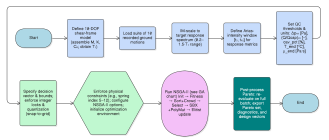
\includegraphics[width=\linewidth]{Genel.pdf}
  \caption{Overall methodological workflow: (Phase 1) input preparation and ground-motion processing, (Phase 2) GA setup and definition of decision variables, objectives and safety constraints, and (Phase 3) optimisation loop and Pareto-front extraction.}
  \label{fig:overall_workflow}
\end{figure}

% Motivasyon, literatürde boşluk, katkılar ve makale organizasyonu.

\section{Methods: Physical \& Numerical Modelling}

\begin{figure}[t]
  \centering
  \includegraphics[width=0.6\textwidth]{sistemcs.pdf}
  \caption{Schematic diagram of the $n$ storey shear frame equipped with a roof level fluid viscous damper (FVD).}
  \label{fig:FVDschematic}
\end{figure}

Figure~\ref{fig:FVDschematic} shows the $n$-DOF shear frame with a roof level FVD considered in this study. We used a detailed numerical model that coupled the $n$-DOF structural dynamics of the frame with the nonlinear thermal and hydraulic behaviour of the damper. In this model we did not rely on simplified phenomenological laws such as $F = C|\dot u|^{\alpha}$. Instead, the FVD submodel was mechanistic and included three main components: (i) orifice hydraulics with a Reynolds dependent discharge coefficient $C_d(\mathrm{Re})$ and jet loss scaling $\Delta p \propto Q^2$ \citep{Yau2017,Hutagalung2019,Osman2019}; (ii) a physics based cavitation limiter implemented as a differentiable soft minimum between the jet candidate and an effective vapour threshold, consistent with orifice cavitation inception criteria \citep{Davoudi2021}; and (iii) a two node thermal block that coupled temperature to viscosity and density, so that both $c_{\mathrm{lam}}(T)$ and $C_d(\mathrm{Re}(T))$ responded to heating \citep{Yau2017,Zhong2020}.

\noindent\textit{Rationale.} Classical $F = C|\dot u|^{\alpha}$ laws lump laminar and jet mechanisms and cannot track pressure, cavitation and thermal safety under pulse type demands. For sharp edged short orifices in the relevant $\mathrm{Re}$ range, $\Delta p$ follows a quadratic $Q$ law with $C_d$ varying with $\mathrm{Re}$ and geometry \citep{Yau2017,Hutagalung2019,Osman2019}. Keeping linear viscous losses in a parallel branch avoids double counting inside the orifice drop. Cavitation onset places a physical cap tied to vapour pressure and local accelerations \citep{Davoudi2021}, and practical FVD design and qualification likewise impose explicit pressure and capacity limits that we carried forward into the quality control metrics \citep{Zhong2020,Acquaro2020SDEE,Song2016ICMS}.

This coupling gave a stiff, coupled system of ordinary differential equations that advanced both the structural degrees of freedom and the damper temperatures at the same time [cite: 331]. We integrated this system with the MATLAB solver \texttt{ode15s}. The relative and absolute tolerances were set to \texttt{RelTol = 1.0e-3} and \texttt{AbsTol = 1.0e-6}, which we found sufficient to stabilise the damper response in the stiffest parts of the motion [cite: 131, 134, 150, 163]. After each analysis, we evaluated all performance and safety metrics (PFA, IDR, pressure, temperature) over the significant duration interval from $t_5$ to $t_{95}$ of the ground motion [cite: 332, 372].

\subsection{Structural model}\label{sec:structural_model}

We modelled a ten storey benchmark frame as a planar shear system with one lateral degree of freedom (DOF) per floor, because the lateral response is dominated by interstorey drift in the first mode. Let $\boldsymbol{x}(t)\in\mathbb{R}^{10}$ denote the relative floor displacements with respect to the moving base, and let $\boldsymbol{r}=\boldsymbol{1}\in\mathbb{R}^{10}$ be the base excitation influence vector. The equations of motion are
\begin{equation}
  \boldsymbol{M}\,\ddot{\boldsymbol{x}}(t)
  + \boldsymbol{C}_0\,\dot{\boldsymbol{x}}(t)
  + \boldsymbol{K}\,\boldsymbol{x}(t)
  + \boldsymbol{f}_{\mathrm{d}}(t)
  =
  -\,\boldsymbol{M}\,\boldsymbol{r}\,a_g(t),
  \label{eq:eom}
\end{equation}
where $\boldsymbol{M}$, $\boldsymbol{C}_0$ and $\boldsymbol{K}$ are the mass, structural damping and stiffness matrices, and $\boldsymbol{f}_{\mathrm{d}}(t)$ collects the nodal forces contributed by the devices. Appendix~\ref{app:derived} lists the storey masses, stiffnesses and damping ratios used to assemble these matrices, together with the modal notation adopted for intensity scaling.

\paragraph{Storey kinematics and device coupling}

We introduce the first difference (incidence) operator $\boldsymbol{B}\in\mathbb{R}^{9\times 10}$ so that
\begin{equation}
  \Delta\boldsymbol{x}(t)=\boldsymbol{B}\,\boldsymbol{x}(t),\qquad
  \Delta\dot{\boldsymbol{x}}(t)=\boldsymbol{B}\,\dot{\boldsymbol{x}}(t),
  \label{eq:drift}
\end{equation}
and storey drift and drift rate follow directly from matrix multiplication. If $\boldsymbol{f}_{\mathrm{story}}(t)\in\mathbb{R}^{9}$ stacks the forces delivered by devices acting between floors, the associated nodal contribution assembles as
\begin{equation}
  \boldsymbol{f}_{\mathrm{d}}(t)=\boldsymbol{B}^{\mathsf T}\,\boldsymbol{f}_{\mathrm{story}}(t).
  \label{eq:fd_assembly}
\end{equation}

\paragraph{Response measures (Arias window)}

Absolute floor accelerations are defined as
\begin{equation}
  \boldsymbol{a}_{\mathrm{abs}}(t)=\ddot{\boldsymbol{x}}(t)+\boldsymbol{r}\,a_g(t),
  \label{eq:aabs}
\end{equation}
and the roof peak floor acceleration (PFA) is evaluated on the Arias window $[t_5,t_{95}]$ as
\begin{equation}
  \mathrm{PFA}=\max_{t\in[t_5,t_{95}]}\big|\,\boldsymbol{e}_{10}^{\mathsf T}\boldsymbol{a}_{\mathrm{abs}}(t)\,\big|.
  \label{eq:PFA}
\end{equation}
For a uniform storey height $h$, the maximum interstorey drift ratio (IDR) is
\begin{equation}
  \mathrm{IDR}=\max_{t\in[t_5,t_{95}]}\left\| \frac{\Delta\boldsymbol{x}(t)}{h} \right\|_{\infty}.
  \label{eq:IDR}
\end{equation}
Details of the tridiagonal assembly of $\boldsymbol{K}$ and $\boldsymbol{C}_0$ from storey parameters, and of the modal notation used for intensity scaling (including the first mode period $T_1$), are given in Appendix~\ref{app:derived}.

\subsection{Damper physics}\label{sec:damper_physics}

\begin{figure}[t]
  \centering
  \includegraphics[width=0.9\linewidth]{ViscousDamper_CAD.pdf}
  \caption{Schematic section of the fluid viscous damper (FVD). The piston head separates Chamber~1 and Chamber~2 and carries the orifices; the working fluid is a compressible silicone oil \citep{wacker:2002:siliconefluids,tamson:2019:siliconoil}, and a coil spring in parallel provides the stiffness $k_{sd}$.}
  \label{fig:damper_schematic}
\end{figure}

The storey device is described by two branches in parallel: a linear elastic branch that collects the overall axial compliance and a hydraulic branch that carries the orifice flow, as indicated in Figure~\ref{fig:damper_schematic}. With the storey drift $\Delta x(t)$ and drift rate $\Delta \dot x(t)$ defined as
\begin{equation}
  \Delta x(t)=x_{i+1}(t)-x_i(t),\qquad 
  \Delta \dot x(t)=\dot x_{i+1}(t)-\dot x_i(t),
  \label{eq:dx-dv}
\end{equation}
and with $A_p$ the piston area and $A_o$ the total orifice area ($A_o=n_{\mathrm{orf}}\pi d_o^2/4$), the storey force is written as
\begin{equation}
  F_{\mathrm{story}}(t)=F_{\mathrm{elastic}}(t)+F_{\mathrm{laminar}}(t)+F_{\mathrm{orifice}}(t),
  \label{eq:Fstory}
\end{equation}
where the elastic and laminar contributions read
\begin{equation}
  F_{\mathrm{elastic}}(t)=k_{sd}\,\Delta x(t),\qquad
  F_{\mathrm{laminar}}(t)=c_{\mathrm{lam}}(T)\,\Delta \dot x(t).
  \label{eq:Felam}
\end{equation}
In the elastic branch, $k_{sd}$ gathers the compliance of the hydraulic assembly and the coil spring; Appendix~\ref{app:derived} reports the geometric relations used to compute this stiffness.

\paragraph{Kinematics, layout and multiplicity}

A positive $\Delta x$ increases the volume of the upper chamber and reduces the volume of the lower chamber, and the associated algebraic flow is counted as positive from the upper side to the lower side. For the ten storey frame considered in Section~\ref{sec:structural_model}, one equivalent damper element with $n_\parallel=1$ is assigned to each of the nine interstorey levels. Section~\ref{sec:opt_ga} varies the damper parameters within this single equivalent layout, so the same parameter set is used for all nine devices. This $n_\parallel=1$ element represents the total hydraulic circuit for that storey. In a practical installation where several physical cylinders act in parallel, their contributions (for example $A_p$, $A_o$, $hA$) are lumped into this equivalent element to avoid redundant design variables. For a regular plan building, the same damper design is adopted for the orthogonal ($Y$) direction.

\subsubsection*{Orifice hydraulics: jet loss with $C_d(\mathrm{Re})$ (no linear drop inside $\Delta p$)}

The safety metric $(Q/Q_{\mathrm{cap}})_{95}$ requires a reference flow capacity for the orifice. We therefore define the theoretical orifice flow capacity under a nominal design pressure cap $\Delta p_{\mathrm{cap}}$ as
\begin{equation}
  Q_{\mathrm{cap}} = C_d^\infty A_o \sqrt{ \frac{2 \,\Delta p_{\mathrm{cap}}}{\rho(T)} }.
  \label{eq:Qcap_def}
\end{equation}
The design pressure cap is taken as
$\Delta p_{\mathrm{cap}}=\phi\,p_{\mathrm{work}}$ with $\phi=1.5$, where $p_{\mathrm{work}}$ is the manufacturer rated maximum working pressure \citep{Eiga2024}. When no project specific rating is available, we set $\Delta p_{\mathrm{cap}}=\SI{20}{MPa}$, which falls in the lower half of the typical range reported for seismic FVD orifices (about 14--69 MPa). This choice gives roughly $1.5$ times the working pressure, in line with hydraulic pressure test practice \citep{Eiga2024}.

The saturated flow used in the jet loss term is
\begin{equation}
  Q_{\mathrm{sat}}(\Delta\dot x)=
  Q_{\mathrm{cap}}\;\tanh\!\Big(\frac{A_p}{Q_{\mathrm{cap}}}\sqrt{\Delta\dot x^{\,2}+v_\varepsilon^{\,2}}\Big),
  \qquad v_\varepsilon>0.
  \label{eq:Qsat}
\end{equation}
Only the quadratic (jet) head loss contributes to the orifice pressure candidate, in line with single phase orifice behavior,
\begin{equation}
  \Delta p_{\mathrm{kv}}(Q_{\mathrm{sat}},T)
  =\frac{\rho(T)\,Q_{\mathrm{sat}}\,|Q_{\mathrm{sat}}|}{2\,[C_d(\mathrm{Re})\,A_o]^2},
  \label{eq:dp-kv}
\end{equation}
which reflects the measured $\Delta p \propto Q^2$ (equivalently $Q\propto\sqrt{\Delta p}$) relationships for sharp, short orifices at relevant Reynolds numbers \citep{Cioncolini2018,Abd2019,Golijanek-Jdrzejczyk2023}. Linear viscous losses act only through the parallel laminar branch $c_{\mathrm{lam}}(T)$ in Eq.~\eqref{eq:Felam}; embedding an additional linear drop inside $\Delta p$ would double count the same mechanism.

The Reynolds number and the discharge coefficient are written as
\begin{equation}
  \mathrm{Re}
  =\frac{\rho(T)\,|Q_{\mathrm{sat}}|\,d_o}{\mu(T)\,A_o},
  \qquad
  C_d(\mathrm{Re})=
  C_d^\infty-\frac{C_d^\infty-C_d^0}{1+\big(\mathrm{Re}/\mathrm{Re}_0\big)^{p_{\exp}}},
  \label{eq:Cd-Re}
\end{equation}
with $C_d$ clamped to admissible bounds. Experiments show that the functional relation between $C_d$ and $\mathrm{Re}$ and the onset of a high Reynolds plateau depend on geometry and operating conditions \citep{laMorena2018,Lee2018,Ahmed2020,Gao2019}. In this study we hold the transition scale fixed at $\mathrm{Re}_0=\num{1000}$ to avoid over parameterization and identifiability issues in the twelve dimensional design space; Appendix Table~\ref{tab:fixed-values-phys} lists this value together with the supporting references.

\paragraph{Laminar equivalent (used outside $\Delta p_{\mathrm{kv}}$)}
For diagnostics and for the explicit viscous branch in Eq.~\eqref{eq:Felam}, the laminar network is represented by its equivalent flow resistance $R_{\mathrm{lam}}$. The resulting laminar coefficient $c_{\mathrm{lam}}$ follows from the standard hydraulic to mechanical equivalence $c_{\mathrm{lam}} = R_{\mathrm{lam}} A_p^2$:
\begin{equation}
  R_{\mathrm{lam}}(T)
  =\frac{128\,\mu(T)\,L_{\mathrm{ori}}}{\pi\,d_o^4}\,\frac{1}{n_{\mathrm{orf}}},
  \qquad
  c_{\mathrm{lam}}(T)=R_{\mathrm{lam}}(T)\,A_p^2,
  \label{eq:Rlam-clam}
\end{equation}
so that $F_{\mathrm{laminar}}(t)=c_{\mathrm{lam}}(T)\,\Delta\dot x(t)$. The resistance $R_{\mathrm{lam}}$ does not enter Eq.~\eqref{eq:dp-kv}; there is no linear drop inside $\Delta p$.

\subsubsection*{Cavitation limiter (physical model)}\label{sec:damper_cav}

Cavitation is handled by applying a smooth lower bound to the orifice pressure. An upstream pressure proxy is obtained from the elastic term relative to ambient:
\begin{equation}
  p_{\uparrow}(t)=p_{\mathrm{amb}}+\frac{|F_{\mathrm{elastic}}(t)|}{A_p}.
  \label{eq:pup}
\end{equation}
Comparing $p_{\uparrow}$ to an effective vapour threshold defines the cavitation limited drop,
\begin{equation}
  \Delta p_{\mathrm{cav}}(t)
  =\max\!\big\{\big(p_{\uparrow}(t)-p_{\mathrm{cav,eff}}\big)\cdot \mathrm{cav\_sf},\,0\big\},
  \label{eq:dpcav}
\end{equation}
and the effective orifice pressure is taken as the differentiable minimum
\begin{equation}
  \Delta p_{\mathrm{eff}}
  =\operatorname{softmin}_{\varepsilon}\!\big(\Delta p_{\mathrm{kv}},\,\Delta p_{\mathrm{cav}}\big).
  \label{eq:softmin}
\end{equation}
The cavitation fraction over the Arias window is the time ratio for which $\Delta p_{\mathrm{kv}}>\Delta p_{\mathrm{cav}}$.

\paragraph{Cavitation threshold (physical basis)}
Room temperature silicone oils have very low vapour pressures (order of $1$ to $2$ Pa), and cavitation inception is strongly influenced by dissolved gas and surface nuclei. Degassing protocols in silicone oil Venturi experiments markedly change inception, which underscores the role of gas content; diffusion driven nucleation from surface nuclei explains why inception can occur at absolute pressures that are still relevant for engineering applications \citep{Croci2020ApplSci,GrossPelz2017JFM}. We therefore set an effective threshold $p_{\mathrm{cav,eff}}$ in the kilopascal range by applying a conservative safety factor above the pure vapour pressure, so that the limiter flags only physically plausible inception in civil scale FVDs.

\paragraph{Smooth minimum for numerical robustness}
To keep the right hand side differentiable for stiff time integration and for gradient based penalties, we use the log sum exp smooth minimum
\[
  \operatorname{softmin}_{\varepsilon}(a,b)
  = -\,\varepsilon \,\log\!\big(\mathrm{e}^{-a/\varepsilon}+\mathrm{e}^{-b/\varepsilon}\big),
\]
which monotonically approaches $\min(a,b)$ as $\varepsilon\downarrow 0$ and removes non physical kinks while preserving the correct limiting behavior \citep{Cuturi2013OTSoftmin}.

\paragraph{Orifice force with smoothed sign}
The hydraulic contribution to the storey force is
\begin{equation}
  F_{\mathrm{orifice}}(t)
  =\Delta p_{\mathrm{eff}}(t)\,A_p\,
  \frac{\Delta\dot x(t)}{\sqrt{\Delta\dot x^{\,2}(t)+v_\varepsilon^{\,2}}}.
  \label{eq:Forf}
\end{equation}

\noindent\textit{Convention.} Linear (laminar) losses act only through $c_{\mathrm{lam}}(T)$ in $F_{\mathrm{laminar}}$; the orifice pressure uses the jet term with cavitation limiting, and no linear drop is embedded in $\Delta p$.

\subsubsection*{Thermal block (coupled viscosity feedback)}

A compact two node energy balance (oil $T_o$, steel or cylinder $T_s$) is advanced concurrently with the structural state. This ensures that the temperature dependent viscosity $\mu(T)$ is updated inside the force evaluation and feeds back immediately into $c_{\mathrm{lam}}(T)$ and the Reynolds dependent $C_d(\mathrm{Re}(T))$:
\begin{align}
  C_o\,\dot T_o &= P_{\mathrm{loss}} - hA_{o\leftrightarrow s}(T_o-T_s) - hA_{o\leftrightarrow \mathrm{env}}(T_o-T_\infty), \label{eq:To}\\
  C_s\,\dot T_s &= \phantom{P_{\mathrm{loss}}}\; +\,hA_{o\leftrightarrow s}(T_o-T_s) - hA_{s\leftrightarrow \mathrm{env}}(T_s-T_\infty). \label{eq:Ts}
\end{align}

To keep the number of thermal parameters manageable, all three exchange coefficients in Eqs.~\eqref{eq:To}--\eqref{eq:Ts} are linked to the single optimization variable $hA$ (total thermal conductance) listed in Table~\ref{tab:opt-vars}. We adopt a lumped model with
\[
  hA_{o\leftrightarrow s} = hA_{o\leftrightarrow \mathrm{env}} = hA_{s\leftrightarrow \mathrm{env}} = hA,
\]
and no additional fixed baseline value is listed in the Appendix.
Consistent with the three term force split, the instantaneous mechanical power is the sum of the laminar and orifice contributions (with no linear drop inside $\Delta p$):
\begin{equation}
   P_{\mathrm{loss}}(t)%
  = \underbrace{c_{\mathrm{lam}}(T_o)\,\Delta\dot x^{\,2}(t)}_{P_{\mathrm{laminar}}}
  + \underbrace{\Delta p_{\mathrm{eff}}(t)\,\left| Q_{\mathrm{sat}}(t) \right|}_{P_{\mathrm{orifice}}}
  \ge 0 .
  \label{eq:Ploss}
\end{equation}

\noindent\textit{Energy transfer and power split.}
The split in Eq.~\eqref{eq:Ploss} follows standard hydraulic energetics. The laminar branch dissipates mechanical power as
$P_{\mathrm{laminar}}=c_{\mathrm{lam}}(T_o)\,\Delta\dot x^{\,2}$,
while the orifice branch converts hydraulic power
$P=\Delta p_{\mathrm{eff}}\,|Q_{\mathrm{sat}}|$ into heat. Their sum gives the mechanical to thermal conversion that drives the two node balance in Eqs.~\eqref{eq:To}--\eqref{eq:Ts}. This is consistent with the mechanical energy balance for short, sharp edged orifices,
$Q=C_d(\mathrm{Re})\,A_o\sqrt{2\,\Delta p/\rho}$, hence $\Delta p\propto Q^{2}$; here $C_d$ depends on $\mathrm{Re}$ at low to intermediate values and approaches a plateau as $\mathrm{Re}$ increases \citep{Yau2017,Cheng2020,Ahmed2020}.

Temperature dependent properties follow smooth laws:
\begin{equation}
  \mu(T)=\mu_{\mathrm{ref}}\,\exp\!\big(b_\mu (T-T_{\mathrm{ref}})\big),
  \qquad
  \rho(T)=\frac{\rho_{\mathrm{ref}}}{1+\alpha_\rho (T-T_{\mathrm{ref}})}.
  \label{eq:props}
\end{equation}

\noindent\textit{Temperature dependent properties.}
For PDMS silicone oils, the viscosity temperature relation is well captured over engineering ranges (roughly $20$ to $100\,^{\circ}$C and low to moderate shear) by log linear or Arrhenius type fits, which motivates the exponential form in Eq.~\eqref{eq:props}. We calibrate the fit around $T_{\mathrm{ref}}=\SI{25}{^\circ C}$ using manufacturer data for the specific oil grade in the zero shear region. The same dataset provides the density slope $\alpha_{\rho}$ used in Eq.~\eqref{eq:props}, so that $\rho(T)$ and therefore $\mathrm{Re}(T)$ and $C_d(\mathrm{Re}(T))$ respond consistently to heating \citep{Swallow2002,Venczel2021,Zhai2019,wacker:2002:siliconefluids,tamson:2019:siliconoil}. The property slopes $b_\mu$, $\alpha_\rho$ and the optional $b_\rho$ in Eq.~\eqref{eq:props} were obtained by least squares fits to the same manufacturer data.

The accumulated dissipation reported on the Arias window is
\begin{equation}
  E_{\mathrm{mech}}
  =\int_{t_5}^{t_{95}} P_{\mathrm{loss}}(t)\,\mathrm{d}t
  =\int_{t_5}^{t_{95}} \!\Big(c_{\mathrm{lam}}(T_o)\,\Delta\dot x^{\,2}(t)
  +\Delta p_{\mathrm{eff}}(t)\,\big|Q_{\mathrm{sat}}(t)\big|\Big)\,\mathrm{d}t .
  \label{eq:Emech}
\end{equation}

\paragraph{Parameters (deferred)}
Appendix~\ref{app:derived} consolidates the fixed coefficients, bounds and geometric data used in the damper model. It includes: (i) the transition parameters for $C_d(\mathrm{Re})$ (with fixed $\mathrm{Re}_0$); (ii) the geometry and elastic or compressibility terms that determine $k_{sd}$; (iii) the constants used in the cavitation limiter; and (iv) the thermal exchange parameters and property slopes. Units follow SI conventions, with $Q$ in \si{m^3\,s^{-1}}, $\Delta p$ in \si{Pa} and areas in \si{m^2}.

\subsection{Time integration}\label{sec:time_integration}

We integrated the coupled frame and damper model with a stiff variable step ODE scheme. The state vector collects the structural displacements and velocities together with the two thermal degrees of freedom, while the hydraulic quantities are evaluated algebraically inside the right hand side. With $\boldsymbol{x}(t)\in\mathbb{R}^{10}$ the relative floor displacements and $\boldsymbol{v}(t)=\dot{\boldsymbol{x}}(t)$, the first order form reads
\[
\boldsymbol{z}(t)=
\begin{bmatrix}
\boldsymbol{x}(t)\\[2pt]
\boldsymbol{v}(t)\\[2pt]
T_o(t)\\[2pt]
T_s(t)
\end{bmatrix},
\qquad
\begin{aligned}[t]
\dot{\boldsymbol{x}}(t)&=\boldsymbol{v}(t),\\
\dot{\boldsymbol{v}}(t)&=
-\,\boldsymbol{M}^{-1}\!\Big(
  \boldsymbol{C}_0\,\boldsymbol{v}(t)
  +\boldsymbol{K}\,\boldsymbol{x}(t)
  +\boldsymbol{f}_{\mathrm{d}}(t)
\Big)
-\boldsymbol{r}\,a_g(t),
\end{aligned}
\]
where $\boldsymbol{f}_{\mathrm{d}}(t)=\boldsymbol{B}^{\mathsf T}\boldsymbol{f}_{\mathrm{story}}(t)$ and $\boldsymbol{f}_{\mathrm{story}}(t)$ is returned by the mechanistic device model from the instantaneous storey drift and drift rate.

\paragraph{Device evaluation within the right hand side}

At each evaluation time, the damper routine forms $\Delta\dot x(t)=\boldsymbol{B}\,\boldsymbol{v}(t)$ and uses the current oil temperature to compute the saturated flow $Q_{\mathrm{sat}}$ (Eq.~\eqref{eq:Qsat}), the Reynolds number and discharge coefficient $C_d(\mathrm{Re})$ (Eq.~\eqref{eq:Cd-Re}), the jet candidate $\Delta p_{\mathrm{kv}}$ (Eq.~\eqref{eq:dp-kv}) and the cavitation limited pressure $\Delta p_{\mathrm{eff}}$ (Eq.~\eqref{eq:softmin}). The storey force is then assembled as the sum of the elastic term, the laminar branch and the orifice contribution with smoothed sign (Eqs.~\eqref{eq:Felam} and \eqref{eq:Forf}).

\paragraph{Ground motion, solver and response window}

The base acceleration $a_g(t)$ is obtained by linear interpolation of the sampled record. Large pressure gradients and the cavitation limiter make the device equations stiff at high velocities, so we used the MATLAB solver \texttt{ode15s} for all runs. The relative and absolute tolerances were set to $\text{RelTol}=1.0\times 10^{-3}$ and $\text{AbsTol}=1.0\times 10^{-6}$; these values stabilised the damper response without excessive step rejection. The solution is evaluated on the native record grid, but response measures are extracted only on the Arias window $[t_5,t_{95}]$ to exclude the start up drift and late coda.

\paragraph{Thermal coupling}

The two node thermal block in Eqs.~\eqref{eq:To}--\eqref{eq:Ts} is advanced together with the structural state and feeds back through $\mu(T_o)$ and $\rho(T_o)$. The mechanical power that drives the thermal balance is $P_{\mathrm{loss}}(t)$ in Eq.~\eqref{eq:Ploss}, and the accumulated dissipation on $[t_5,t_{95}]$ is $E_{\mathrm{mech}}$ in Eq.~\eqref{eq:Emech}.

\paragraph{Initial conditions and masks}

The frame starts from rest, with $\boldsymbol{x}(t_0)=\boldsymbol{0}$ and $\boldsymbol{v}(t_0)=\boldsymbol{0}$. Device multiplicity and storey activity masks are applied algebraically: areas and linear coefficients scale with $n_\parallel$, and inactive storeys are set to zero. This keeps the assembled system sparse and avoids modifying the core integrator. Additional numerical safeguards, such as the soft minimum sharpness and the small velocity regularisation in Eq.~\eqref{eq:Forf}, are listed in Appendix~\ref{app:derived}.

\subsection{Ground motion processing and scaling}

We used a set of ten recorded horizontal ground motions for all nonlinear analyses. Each accelerogram was converted to SI units (m/s$^2$) and de trended, and a mild high pass filter (for example $f_c=0.05$~Hz) was applied when baseline drift was visible [cite: 340].

To place all records at a common intensity level, each motion was scaled to a target intensity $\mathrm{IM}_\star$. The chosen measure is the band averaged geometric mean of the 5\% damped pseudo spectral acceleration, evaluated on $N$ linearly spaced periods within a band centred on the first mode period $T_1$, from $T_1/\gamma$ to $\gamma T_1$:
\begin{equation}
\mathrm{IM}_{\mathrm{band}}=\exp\!\left(\frac{1}{N}\sum_{k=1}^{N}\ln S_a^{(5\%)}(T_k)\right), 
\qquad T_k \in [T_1/\gamma,\ \gamma T_1].
\label{eq:IMband}
\end{equation}
This band averaged quantity belongs to the family of $S_a$ based measures that work with logarithmic ordinates over a period band. By centring the band on $T_1$ it remains efficient and reasonably sufficient for first mode dominated shear frames, and it is directly comparable to Sa,avg or AvSv type measures used in record selection and scaling \citep{Vargas-Alzate2022}. The Arias window $[t_5,t_{95}]$ is used consistently when computing peak or percentile response measures, in line with significant duration definitions based on $D_{5\text{--}95}$ \citep{Davatgari-Tafreshi2023,Jiang2025}.

For each record, the scale factor
\[
s=\frac{\mathrm{IM}_\star}{\mathrm{IM}_{\mathrm{band}}},
\]
clamped to the admissible range $[0.2,\,2.2]$, is applied to obtain the scaled motion $\tilde a_g(t)=s\,a_g(t)$. The same scaled input is used for the bare frame and for all damper configurations, so that differences in response stem from the device design rather than from changes in the excitation.

All performance measures (for example PFA, IDR and the damper level safety metrics) are evaluated on the 5\%--95\% Arias intensity window $[t_5,t_{95}]$. For each design, per record quantities are then averaged over the ten motions to form the optimisation objectives.

\begin{table}[!t]
\centering\footnotesize
\caption{Selected earthquake records used in this study (horizontal components).}
\label{tab:gm-list}
\setlength{\tabcolsep}{6pt}
\renewcommand{\arraystretch}{1.12}
\begin{tabularx}{\linewidth}{@{} 
    l        % Code
    L        % Earthquake name  (esnek, soldan hizalı)
    S[table-format=4.0] % Year
    L        % Station / Component (esnek, soldan hizalı)
    S[table-format=1.1] % Mw
    S[table-format=2.2] % Distance
    S[table-format=1.3] % PGA
@{}}
\toprule
Code & Earthquake name & {Year} & Station / Component & {$M_w$} & {Distance (km)} & {PGA (g)} \\
\midrule
KB95 & Kobe & 1995 & KJMA / KJMA-000                   & 6.9 & 0.96  & 0.833 \\
NR94 & Northridge & 1994 & Sylmar County Hospital / 360 & 6.7 & 9.90  & 0.842 \\
IR80 & Irpinia (Italy) & 1980 & Sturno (STN) / STU270    & 6.9 & 6.78  & 0.320 \\
MJ90 & Manjil & 1990 & Abbar / ABBAR-L                 & 7.3 & 12.55 & 0.510 \\
LP89 & Loma Prieta & 1989 & Calaveras Reservoir / CLR180& 6.9 & 35.28 & 0.110 \\
CC99 & Chi--Chi & 1999 & TCU078 / 90$^\circ$            & 7.6 & 8.30  & 0.442 \\ % 433.6 cm/s^2 → 0.442 g
MR23 & Kahramanmaras (Türkiye) & 2023 & TK~4614 / HNE   & 7.8 & 9.80  & 2.209 \\ % 2166.435 cm/s^2 → 2.209 g
TB78 & Tabas & 1978 & Tabas / H2                        & 7.4 & 2.10  & 0.862 \\
CM92 & Cape Mendocino & 1992 & Petrolia / H2             & 7.0 & 8.20  & 0.662 \\
CH07 & Chuetsu & 2007 & Joetsu Kakizaki / 65010EW      & 6.8 & 9.43  & 0.580 \\
\bottomrule
\end{tabularx}

\vspace{1pt}
{\RaggedRight\scriptsize
Sources: PEER NGA-West2 (all but MR23) and AFAD Strong Motion Databases (MR23).
Distances use closest-to-fault values ($R_{\mathrm{rup}}$) when available and all PGA entries are reported in $g$; Chi--Chi and Kahramanmaras were converted from cm/s$^2$ using $1\,g=980.665$~cm/s$^2$.
Codes coincide with the internal labels used in the optimisation runs (MR23 corresponds to AFAD TK~4614, HNE component), and the mix intentionally retains high-PGA near-fault motions (for example MR23 at \SI{2.209}{g}) to exercise the pressure, temperature and cavitation limits enforced by the QC metrics.
\par}
\end{table}
\FloatBarrier

\section{Optimization Framework}\label{sec:opt_ga}

% --- REVİZYON: Metin paragrafı, figürden önceye taşındı ---
We solved a safety first lexicographic multi objective problem. Candidate designs were ranked by
\(\big[f_{\mathrm{pen}},\, f_1{=}\langle\mathrm{PFA}\rangle,\, f_2{=}\langle\mathrm{IDR}\rangle\big]\), and we examined the Pareto trade off in \((f_1,f_2)\) for solutions with \(f_{\mathrm{pen}}\approx 0\).
Figure~\ref{fig:ga_flowchart} sketches the workflow. The aim was to identify device parameters \(\boldsymbol{d}\) that reduce the record mean roof peak floor acceleration (PFA) and the record mean maximum interstorey drift ratio (IDR) at the same time. These metrics were evaluated on the Arias window responses \([t_5,t_{95}]\) for a fixed set of ten intensity scaled ground motions.

% --- REVİZYON: Figür, metinden sonraya taşındı ---
\begin{figure}[!htbp]
  \centering
  % REVİZYON: Figür, sayfaya sığması için küçültüldü
  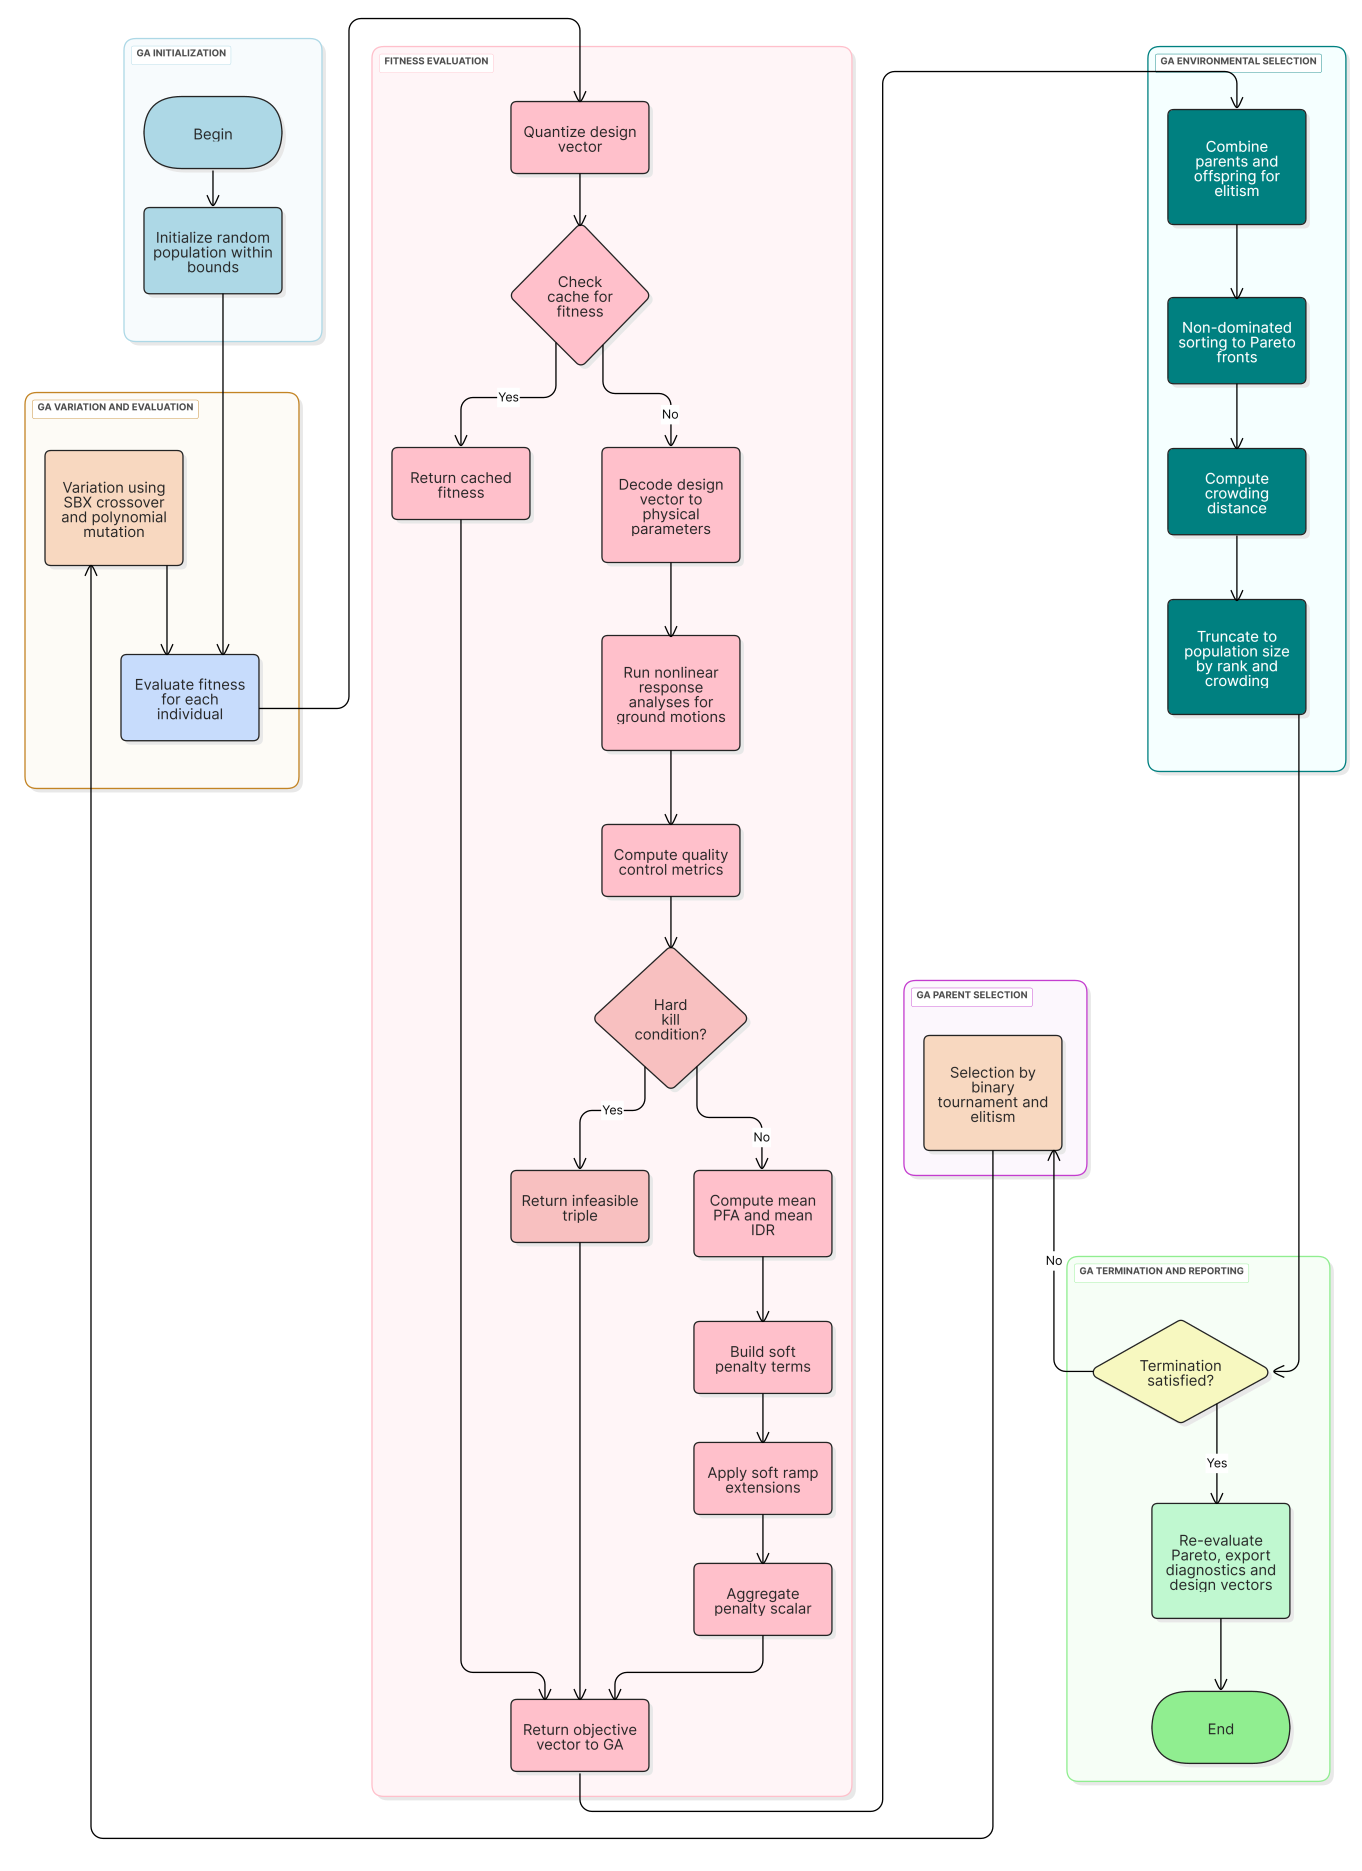
\includegraphics[width=0.72\linewidth]{GA.pdf}
  \caption{Flowchart of the NSGA-II optimization process, illustrating population evaluation, safety screening (hard constraints), and multi objective ranking ($f_{\mathrm{pen}}, f_1, f_2$).}
  \label{fig:ga_flowchart}
\end{figure}

% \FloatBarrier komutu kaldırıldı.

\subsection{Objectives and Safety Constraints}\label{sec:opt_obj}
The primary performance objectives are the record wise arithmetic means of the structural demands:
\begin{equation}
\min_{\boldsymbol{d}\in\mathcal{X}} \quad
f_1(\boldsymbol{d})=\frac{1}{10}\sum_{j=1}^{10}\mathrm{PFA}_j(\boldsymbol{d}),
\qquad
f_2(\boldsymbol{d})=\frac{1}{10}\sum_{j=1}^{10}\mathrm{IDR}_j(\boldsymbol{d}) ,
\label{eq:obj_main}
\end{equation}
where $\mathcal{X}$ is the admissible (manufacturable and physically valid) design space.

Hydraulic and thermal safety is enforced using a two tier policy. First, a hard screen discards any design that violates the fixed thresholds (see boxed text) on any record. Second, feasible designs are ranked lexicographically using the vector
\[
\big[\,f_{\mathrm{pen}},\; f_1,\; f_2\,\big].
\]
This ordering puts safety in front of the structural objectives. The penalty function $f_{\mathrm{pen}}$ is a smooth aggregate of normalised safety excesses; it is zero when all checks are satisfied and increases monotonically with any near violation, while remaining differentiable for the solver.

\noindent\fbox{%
\parbox{\dimexpr\linewidth-2\fboxsep-2\fboxrule\relax}{%
\textbf{Fixed QC thresholds (per record, on Arias window).}
\begin{itemize}
    \item Max. 95th percentile pressure: $\Delta p_{95}\le \SI{4.0e7}{Pa}$
    \item Max. 95th percentile flow ratio: $(Q/Q_{\mathrm{cap}})_{95}\le 0.90$
    \item Max. cavitation time fraction: $\mathrm{cav}_{\mathrm{pct}} \le 0.5\%$
    \item Max. end of window temperature: $T_{\mathrm{end}}\le \SI{75}{\celsius}$
    \item Min. end of window viscosity: $\mu_{\mathrm{end}}\ge \SI{0.70}{Pa.s}$
\end{itemize}
}}

\par
The thresholds in the QC box were set conservatively to match the operating envelope of industrial FVDs and to balance device longevity, model validity and material constraints. They are deliberately strict and consistent with the safety first ordering of objectives.

We motivate the main limits as follows.
(i) The internal pressure bound ($\Delta p_{95}\le \SI{4.0e7}{Pa}$, about \SI{40}{MPa}) was chosen to preserve the mechanical integrity of the cylinder and seals. For comparison, high performance damper seals are rated up to roughly \SI{275}{MPa}, and burst tests for civil devices often target pressures on the order of \SI{140}{MPa} \cite{TaylorDevices2024}.
(ii) The thermal limits ($T_{\mathrm{end}}\le \SI{75}{\celsius}$ and $\mu_{\mathrm{end}}\ge \SI{0.70}{Pa.s}$) serve a dual purpose. They keep the device within the functional range reported for silicone fluid dampers (typically from about $-40$ to $+70\,^\circ$C) \cite{MDPI_Thermal2023} and avoid excessive thermal thinning or degradation, which becomes more likely above roughly \SI{90}{\celsius}. In this way the calibrated $\mu(T)$ and $C_d(\mathrm{Re}(T))$ relations remain valid.
(iii) The flow ratio cap ($(Q/Q_{\mathrm{cap}})_{95}\le 0.90$) leaves a ten percent headroom below the nominal orifice capacity. This margin keeps the device away from a choked regime in which compressibility or cavitation dominate and the response becomes highly nonlinear \cite{crane:1982:flowfluids}.
(iv) The cavitation policy ($\mathrm{cav}_{\mathrm{pct}} \le 0.5\%$) replaces an unrealistically strict zero tolerance requirement by a small, practical allowance that is insensitive to minor numerical noise. Cavitation is counted only when the pressure stays below the effective threshold $p_{\mathrm{cav,eff}}$ by at least \SI{0.5}{kPa} for a holding time of \SI{5}{ms} or longer. This de minimis allowance means that brief numerical spikes are ignored, whereas any design that triggers sustained inception and cumulative damage or performance degradation \cite{sist:2018:en15129} is still removed by the hard screen.

Designs breaching any bound are rejected by the hard screen; others are penalised softly via $f_{\mathrm{pen}}$.

\paragraph{Fairness across records}
To ensure fairness, every candidate design $\boldsymbol{d}$ is evaluated against the same set of ten pre scaled ground motions and identical modelling and integration policies. No per record retuning is allowed, so the objective values reflect only changes in the device parameters. While the optimisation uses means, response dispersion is reported in Section~\ref{sec:results} to support robust engineering choices.

\subsection{Decision Variables and Bounds}\label{sec:opt_vars}
The design vector $\boldsymbol{d}$ collects the twelve key parameters that control the hydraulic, elastic and thermal behaviour of the device:
\[
\boldsymbol{d}=\big[
d_o,\ n_{\mathrm{orf}},\ C_d^{0},\ C_d^{\infty},\ p_{\exp},\ L_{\mathrm{ori}},\ hA,\ D_p,\ d_w,\ D_m,\ n_{\mathrm{turn}},\ \mu_{\mathrm{ref}}
\big]^{\mathsf T},
\]
where $d_o$ is the orifice diameter, $n_{\mathrm{orf}}$ the number of parallel orifices (integer), $(C_d^{0},C_d^{\infty},p_{\exp})$ the discharge law parameters, $L_{\mathrm{ori}}$ the orifice length, $hA$ the total heat transfer conductance, $(D_p,d_w,D_m,n_{\mathrm{turn}})$ the piston and spring geometry (with $n_{\mathrm{turn}}$ integer), and $\mu_{\mathrm{ref}}$ the reference viscosity.

The feasible region $\mathcal{X}$ is a box constrained domain (Table~\ref{tab:opt-vars}) with integrality enforced on $n_{\mathrm{orf}}$ and $n_{\mathrm{turn}}$. Bounds in Table~\ref{tab:opt-vars} reflect manufacturability and basic physics. The lower orifice diameter bound avoids sub millimetre drilling that would otherwise require EDM or laser processes and compromised tolerances, while the selected $L_{\mathrm{ori}}/d_o$ range keeps the device in a short, sharp edged orifice tube regime where $C_d(\mathrm{Re})$ exhibits a clear plateau and a predictable sensitivity to thickness and length to diameter ratio \citep{Abdelrahman2021,Jankowski2008,Simpson2018}. Spring geometry enforces a practical spring index $C=D_m/d_w$ in the conventional design range, supported by recent numerical and failure analyses of low index helical springs, to avoid buckling, excessive stress concentrations and premature fatigue \citep{Holschuh2015,Tan2020,Michalczyk2024,Yetgin2024}. Integer constraints on $n_{\mathrm{orf}}$ and $n_{\mathrm{turn}}$ encode the physical multiplicity of orifices and active coils, while piston diameter bounds follow standard seal availability and machining constraints in industrial hydraulic cylinders.

\begin{table}[htbp]
  \centering\footnotesize
  \setlength{\tabcolsep}{2pt}
  \caption{Optimization decision variables and bounds.}
  \label{tab:opt-vars}
  \begin{tabularx}{\linewidth}{@{}>{\RaggedRight\arraybackslash}p{0.16\linewidth}%
    >{\RaggedRight\arraybackslash}X%
    >{\centering\arraybackslash}p{0.14\linewidth}%
    >{\centering\arraybackslash}p{0.14\linewidth}%
    >{\RaggedRight\arraybackslash}p{0.18\linewidth}@{}}
  \toprule
  Symbol & Description & {Lower} & {Upper} & Units \\
  \midrule
  $d_o$           & Orifice diameter (per orifice)        & \num{0.00080} & \num{0.00350} & \si{m} \\
  $n_{\mathrm{orf}}$ & Parallel orifices \textit{(integer)}  & \num{3} & \num{12} & -- \\
  $C_d^{0}$       & Discharge coefficient: laminar limit   & \num{0.55} & \num{0.95} & -- \\
  $C_d^{\infty}$  & Discharge coefficient: turbulent limit & \num{0.70} & \num{1.00} & -- \\
  $p_{\exp}$      & $C_d(\mathrm{Re})$ transition exponent & \num{0.90} & \num{1.60} & -- \\
  $L_{\mathrm{ori}}$ & Orifice length                      & \num{0.10} & \num{0.24} & \si{m} \\
  $hA$            & Total thermal conductance              & \num{150} & \num{400} & \si{W\,K^{-1}} \\
  $D_p$           & Piston diameter                        & \num{0.110} & \num{0.260} & \si{m} \\
  $d_w$           & Spring wire diameter                   & \num{0.008} & \num{0.020} & \si{m} \\
  $D_m^{\dagger}$ & Spring mean diameter                   & \num{0.080} & \num{0.200} & \si{m} \\
  $n_{\mathrm{turn}}$ & Active spring turns \textit{(integer)} & \num{6} & \num{15} & -- \\
  $\mu_{\mathrm{ref}}$ & Reference viscosity at $T_{\mathrm{ref}}$ & \num{0.60} & \num{2.00} & \si{Pa\,s} \\
  \bottomrule
  \end{tabularx}
  \setlength{\tabcolsep}{6pt}% restore default spacing
  \par\vspace{0.3em}\noindent\footnotesize\emph{Manufacturability note.} Bounds enforce drillable orifice diameters, short sharp edged orifice tube aspect ratios, practical spring index and seal compatible piston sizes. $^{\dagger}$Spring index defined as $C=D_m/d_w$.
\end{table}

\paragraph{Search strategy and audit}
The bi objective optimisation problem was solved with a Pareto based evolutionary solver of the NSGA II class. The algorithm used a population of 600 individuals and ran for 180 generations, and each candidate was evaluated over the full ground motion set. We adopted a crossover fraction of $0.90$ with simulated binary crossover and Gaussian mutation (\texttt{MutationFcn=\@mutationgaussian}). The random seed was fixed (\texttt{rng(42,'twister')}) so that the reported Pareto fronts and safety statistics can be reproduced.

After convergence, every non dominated design was re evaluated to collect extended safety and energy indicators (for example, pressure percentiles and energy partitions). These diagnostics were archived and form the basis of the analysis in Section~\ref{sec:results}.

\section{Results and Discussion}\label{sec:results}

This section reports the outcome of the multi-objective optimization and compares the \textbf{Bare Frame} (no dampers) with the \textbf{Optimized System}, defined as the knee-selected FVD from the Pareto front. The focus is on how the optimized device reshapes the seismic demand profile, how it redistributes input energy between structure and damper, and whether it remains within the imposed safety margins.

\subsection{Evaluation of Seismic Performance Enhancement}

Figures~\ref{fig:top-acc}--\ref{fig:max-idr} compare the Arias-window responses for the Bare Frame and the Optimized System. Across all ten records, the optimized configuration suppresses roof absolute acceleration and inter-storey drift. In other words, a larger share of the input energy is absorbed and dissipated within the dampers instead of being stored and repeatedly released in the frame.

\begin{figure}[t]
  \centering
  \includegraphics[width=0.95\linewidth]{Ust_Kat_Mutlak_Ivme_acc_matrix.pdf}
  \caption{Top–floor absolute acceleration over the Arias window (Bare Frame vs. Optimized FVD).}
  \label{fig:top-acc}
\end{figure}

\begin{figure}[t]
  \centering
  \includegraphics[width=0.95\linewidth]{Ust_Kat_Yer_Degistirme_acc_matrix.pdf}
  \caption{Top–floor displacement over the Arias window (Bare Frame vs. Optimized FVD).}
  \label{fig:top-disp}
\end{figure}

\begin{figure}[t]
  \centering
  \includegraphics[width=0.95\linewidth]{Maksimum_IDR_acc_matrix.pdf}
  \caption{Storey–wise maximum inter–storey drift ratio (Bare Frame vs. Optimized FVD).}
  \label{fig:max-idr}
\end{figure}

The visual trends are condensed in Table~\ref{tab:perf-summary}. Record-averaged performance is taken from the post-optimization audit (Section~\ref{sec:opt_ga}): the Baseline row corresponds to the bare frame, and the Optimized row to the knee-selected design obtained from the Pareto set. Percentage gains are reported as
\[
\Delta(\%) \;=\; 100\,\frac{B-O}{B},
\]
where $B$ and $O$ denote the baseline and optimized values of each response metric.

\begin{table}[htbp]
\centering\small
\caption{Record-averaged performance: Bare Frame vs. knee-selected Optimized FVD (from audit).}
\label{tab:perf-summary}
\begin{tabularx}{\linewidth}{@{}>{\RaggedRight\arraybackslash}X*{4}{>{\centering\arraybackslash}X}@{}}
\toprule
Design & $\overline{\mathrm{PFA}}$ [\si{m/s^2}] & $\overline{\mathrm{IDR}}$ [\%] & $\Delta\mathrm{PFA}$ [\%] & $\Delta\mathrm{IDR}$ [\%]\\
\midrule
Baseline (Bare Frame) & \num{13.27} & \num{0.880} & -- & --\\
Optimized (Knee--FVD)  & \num{5.05}  & \num{0.300} & \num{61.9} & \num{65.9}\\
\bottomrule
\end{tabularx}
\end{table}

On this record set, the mean roof acceleration falls from \SI{13.27}{m/s^2} to \SI{5.05}{m/s^2}, which corresponds to a reduction of roughly $60\%$. The mean maximum inter-storey drift ratio decreases from $0.88\%$ to $0.30\%$ (about $65\%$). These reductions are broadly uniform along the height of the building rather than being concentrated at a single storey, which is consistent with the first-mode-dominated response of the ten-storey frame.

\subsection{Multi-Objective Trade-off Analysis and Safety Verification}

Figure~\ref{fig:pareto} displays the final non-dominated set in the objective space $\big(f_1{=}\langle\mathrm{PFA}\rangle,\, f_2{=}\langle\mathrm{IDR}\rangle,\, f_{\mathrm{pen}}\big)$. Many designs lie close to $f_{\mathrm{pen}}\approx 0$, indicating that a sizeable fraction of the Pareto front already satisfies the safety policy of Section~\ref{sec:opt_obj}. Within this feasible cluster, the marked knee solution offers a compromise between reducing structural demands and maintaining device-level margins.

\begin{figure}[t]
\centering
\includegraphics[width=0.82\linewidth]{pareto_front.pdf}
\caption{NSGA–II Pareto front in $(f_1, f_2, f_{\mathrm{pen}})$; the star marks the knee–selected design.}
\label{fig:pareto}
\end{figure}

Knee selection is carried out on the safe part of the front by first retaining only non-dominated designs with $f_{\mathrm{pen}}\approx 0$ and then working in the min--max normalised $(f_1,f_2)$ plane spanned by this subset. In that reduced space, the chosen configuration is the point with the smallest Euclidean distance to the utopian corner $(0,0)$ under equal weights on the two objectives, so the selected design sits near the elbow of the Pareto cloud without favouring either PFA or IDR a priori.

While Table~\ref{tab:perf-summary} summarises the objective values, Table~\ref{tab:safety-verification} lists detailed safety indicators, energy partitions, and peak responses for the selected configuration, including roof displacement and acceleration. Table~\ref{tab:optimized-params} reports the corresponding FVD parameters; in the discussion below, only a subset of these values is used to interpret the safety margins and the energy split.

\begin{table}[htbp]
\centering\small
\caption{Knee-selected design: detailed safety, energy, and peak response indicators (from re-evaluation audit).}
\label{tab:safety-verification}
\resizebox{\linewidth}{!} & {$T_{\mathrm{end}}$ [\si{\celsius}]} & {$\mu_{\mathrm{end}}$ [\si{Pa.s}]} & {$E_{\mathrm{orifice}}$ [\si{J}]} & {$E_{\mathrm{struct}}$ [\si{J}]} & {$P_{\mathrm{mech}}$ [\si{W}]} & {$E_{\mathrm{ratio}}$}\\
\midrule
Knee–FVD (Xbest) &
0.0517 & 7.6273 &
5.98e6 & 0.634 & 0.00 &
74.1 & 0.70 &
3.52e7 & 2.15e7 & 1.48e6 & 1.63\\
\bottomrule
\end{tabular}}
\end{table}

\begin{table}[htbp]
\centering\small
\caption{Optimized design parameters for the knee-selected FVD (corresponds to Table~\ref{tab:safety-verification}).}
\label{tab:optimized-params}
\begin{tabular}{l l c l}
\toprule
Symbol & Parameter & {Value} & Unit \\
\midrule
$d_o$              & Orifice diameter                 & {0.00140} & \si{m} \\
$n_{\mathrm{orf}}$ & Parallel orifices \textit{(int)} & {11}      & -- \\
$C_d^{0}$          & Discharge coeff. (laminar)       & {0.89}    & -- \\
$C_d^{\infty}$     & Discharge coeff. (turbulent)     & {0.77}    & -- \\
$p_{\exp}$         & $C_d(\mathrm{Re})$ transition exp. & {1.46}  & -- \\
$L_{\mathrm{ori}}$ & Orifice length                   & {0.185}   & \si{m} \\
$hA$               & Total thermal conductance        & {228}     & \si{W\,K^{-1}} \\
$D_p$              & Piston diameter                  & {0.157}   & \si{m} \\
$d_w$              & Spring wire diameter             & {0.014}   & \si{m} \\
$D_m$              & Spring mean diameter             & {0.125}   & \si{m} \\
$n_{\mathrm{turn}}$& Active spring turns \textit{(int)}& {10}     & -- \\
$\mu_{\mathrm{ref}}$ & Reference viscosity             & {1.46}    & \si{Pa.s} \\
\bottomrule
\end{tabular}
\end{table}

\paragraph{Safety verification.}

When the configuration in Table~\ref{tab:optimized-params} is re-evaluated on the full ground-motion set, it satisfies all constraints listed in Section~\ref{sec:opt_obj}. As reported in Table~\ref{tab:safety-verification}, the $95$th percentile pressure is about $6\times 10^{6}\,\si{Pa}$, which leaves a substantial margin below the \SI{4.0e7}{Pa} cap chosen to protect seals and barrel under repeated loading. The flow-ratio indicator $Q_{\mathrm{cap95}}\approx 0.63$ remains under the $(Q/Q_{\mathrm{cap}})_{95}\le 0.90$ bound, so the orifice does not operate near its capacity limit for any record in the set. Under the adopted cavitation definition, the time fraction with $p<p_{\mathrm{cav,eff}}$ is essentially zero, indicating that the device does not enter sustained cavitating regimes over the significant duration. The end-of-window temperature $T_{\mathrm{end}}$ stays below \SI{75}{\celsius}, and the final viscosity $\mu_{\mathrm{end}}=\SI{0.70}{Pa.s}$ coincides with the imposed lower limit, keeping the operation within the calibrated range of the $\mu(T)$ and $C_d(\mathrm{Re}(T))$ laws rather than relying on an excessively thinned fluid.

\paragraph{Energy dissipation mechanism.}

The audit also clarifies how the damper reshapes the energy path. Over the Arias window, the orifice branch dissipates on the order of \SI{3.5e7}{J}, whereas the structural contribution is about \SI{2.2e7}{J}. The resulting energy ratio $E_{\mathrm{ratio}}\approx 1.6$ therefore favours the device: more seismic input is converted into heat inside the FVD than is cycled as recoverable strain energy in the frame. This shift in the energy split is consistent with the large reductions in $\langle\mathrm{PFA}\rangle$ and $\langle\mathrm{IDR}\rangle$ reported in Table~\ref{tab:perf-summary}.

\paragraph{Summary.}

The safety-first lexicographic search yields a dense set of feasible designs with $f_{\mathrm{pen}}\approx 0$. Within this set, the selected FVD configuration achieves substantial record-averaged reductions in $\langle\mathrm{PFA}\rangle$ and $\langle\mathrm{IDR}\rangle$ (Table~\ref{tab:perf-summary}) while remaining within all pressure, flow-capacity, cavitation and thermal limits of the coupled model (Table~\ref{tab:safety-verification}). Taken together, the demand, safety and energy indicators suggest that the device operates away from marginal regimes, so the knee design provides a realistic starting point for further engineering refinement and eventual hardware implementation.

\section{Conclusions}

This paper has introduced a high-fidelity modelling and multi-objective design framework for fluid viscous dampers (FVDs) installed on a ten storey shear frame. The model couples a mechanistic FVD description, with a Reynolds dependent discharge coefficient, a cavitation soft limiter and a two node thermal block with temperature dependent viscosity and density, directly to the structural equations of motion; in this way it goes beyond the classical $F = C \lvert v \rvert^{\alpha}$ laws and tracks pressure, flow and temperature histories explicitly \citep{Yau2017,Hutagalung2019,Davoudi2021,Zhong2020}. Seismic demand is represented by ten recorded horizontal ground motions scaled to a common band averaged geometric mean PSA centred on the fundamental period $T_1$, and all response and safety metrics are evaluated on the Arias intensity window $[t_5,t_{95}]$; the record set is deliberately enriched with near fault, high PGA events to probe robustness \citep{Vargas-Alzate2022,Davatgari-Tafreshi2023,Jiang2025}. On top of this physical model, an NSGA-II search with safety first lexicographic ranking, $\big[f_{\mathrm{pen}},\langle\mathrm{PFA}\rangle,\langle\mathrm{IDR}\rangle\big]$, and fixed hydraulic and thermal QC thresholds links device parameters to safe, performance optimised FVD designs.

For the selected configuration, the record mean roof PFA drops from $13.27$ to $5.05~\si{m/s^2}$ (about $60\%$), and the record mean maximum inter storey drift ratio from $0.88\%$ to $0.30\%$ (about $65\%$) over the ten intensity scaled motions (Table~\ref{tab:perf-summary}). Roof displacements and accelerations stay in a moderate range even for the most demanding near fault input, represented here by the Kahramanmara\c{s} MR23 record with a PGA of $2.209~g$; this record still gives controlled response, which is encouraging for a velocity dependent device (Table~\ref{tab:gm-list}) \citep{Song2016ICMS,Acquaro2020SDEE}. An energy audit shows that the orifice branch dissipates about $3.5\times 10^{7}~\si{J}$ per analysis, compared with roughly $2.2\times 10^{7}~\si{J}$ in the structural viscous branch; the resulting ratio $E_{\mathrm{ratio}}\approx 1.6$ means that a clear majority of the seismic input is turned into heat in the damper rather than being cycled through the frame (Table~\ref{tab:safety-verification}). Across the feasible front, many non dominated designs achieve comparable reductions in $\langle\mathrm{PFA}\rangle$ and $\langle\mathrm{IDR}\rangle$ with nearly zero penalty, so the gains seen for the knee solution belong to a broader region of the design space instead of a single finely tuned point (Figure~\ref{fig:pareto}).

The mechanical separation between laminar and orifice branches helps to read the internal energy path of the device. In the knee selected design, the orifice jet loss term carries most of the dissipation, while the laminar branch regulates low velocity behaviour and adds a smaller, but non negligible, share to the thermal load; this picture is consistent with the power split
\[
P_{\mathrm{loss}} = c_{\mathrm{lam}}(T_o)\,\Delta\dot x^{2} + \Delta p_{\mathrm{eff}}\,\lvert Q_{\mathrm{sat}}\rvert
\]
in Eq.~\eqref{eq:Ploss} and with the audit in Table~\ref{tab:safety-verification}. The coupled thermal block raises the oil temperature to $T_{\mathrm{end}}\approx 74~^{\circ}\mathrm{C}$ with a terminal viscosity $\mu_{\mathrm{end}}\approx 0.70~\si{Pa.s}$; this shift increases the Reynolds number and moves $C_d(\mathrm{Re})$ towards its high $\mathrm{Re}$ plateau, but stays within the imposed viscosity bound and within published property trends for PDMS silicone oils. At the same time, the pressure and capacity indicators remain within their prescribed limits, with $dP95\approx 6\times 10^{6}~\si{Pa}$ against a $40~\si{MPa}$ cap and $(Q/Q_{\mathrm{cap}})_{95}\approx 0.63<0.90$, and the cavitation time fraction stays below $0.5\%$ of the Arias window under the adopted definition (Tables~\ref{tab:fixed-values-qc} and~\ref{tab:safety-verification}) \citep{Cioncolini2018,Abd2019,Golijanek-Jdrzejczyk2023,Croci2020ApplSci}. Taken together, these results suggest that, when sized within a physically consistent thermal and hydraulic window, civil scale FVDs can operate safely and efficiently under strong impulsive demands without resorting to unrealistically high viscosities or excessively stiff springs, in line with recent experimental observations on seismic dampers.

From an engineering standpoint, the optimized device sits in the middle of the explored design space and combines a moderate piston diameter, a relatively large number of small orifices, an intermediate reference viscosity and an intermediate thermal conductance. This mix yields substantial response reduction while keeping pressure and temperature in a conservative range (Table~\ref{tab:optimized-params}). In practical design terms, the framework can act as a physics based complement to code oriented procedures: for a chosen building archetype an engineer may fix a target IM band level, set application specific QC thresholds (for example, consistent with EN~15129 limits), and then use a multi objective search to map out a family of safe and efficient FVD designs that can later be condensed into design charts or surrogate models for routine use \citep{sist:2018:en15129,TaylorDevices2024}. The present work, however, is restricted to a planar, first mode dominated ten storey shear frame with a single damper configuration and a fixed set of ten horizontal records; torsional response, three dimensional irregularities, multi directional excitation and multiple damper layouts are not considered, and the damper properties are calibrated to a single family of silicone oils without explicitly modelling manufacturing tolerances, ageing or variability in gas content \citep{Croci2020ApplSci,wacker:2002:siliconefluids}. Future work should address these limitations by validating the coupled thermal and hydraulic model against prototype tests, extending the framework to three dimensional building archetypes and semi active valve laws, and incorporating life cycle cost, ageing and maintenance metrics into the objective set, so that structural safety, device durability and economic performance can be optimised jointly within a performance based design loop.


%% -------------- Back matter --------------
\section*{Data availability}
% Veri/kod erişimi (ör. Zenodo/GitHub bağlantıları).

\section*{CRediT authorship contribution statement}
% ...

\section*{Declaration of competing interest}
% ...

\section*{Acknowledgments}
% ...

%% --- Appendices (place before the bibliography) ---
\appendix
\section{Supplementary symbols and derived quantities}\label{app:derived}
\setcounter{table}{0}
\renewcommand{\thetable}{A.\arabic{table}}
\renewcommand{\theHtable}{A\arabic{table}}

% --- TABLO A.1 ---
\begin{table}[htbp]
\centering\small
\caption{Core structural and coupling symbols (definitions and SI units).}
\label{tab:symbols}
\begin{tabularx}{\linewidth}{@{}>{\RaggedRight\arraybackslash}p{0.18\linewidth}>{\RaggedRight\arraybackslash}p{0.23\linewidth}>{\RaggedRight\arraybackslash}p{0.17\linewidth}>{\RaggedRight\arraybackslash}X@{}}
\toprule
Symbol & Name & Units & Brief definition \\
\midrule
$\boldsymbol{M},\boldsymbol{C}_0,\boldsymbol{K}$ & mass, viscous, stiffness & kg; \si{N.s.m^{-1}}; \si{N.m^{-1}} & Structural operators in Eq.~\eqref{eq:eom}.\\
$\boldsymbol{x},\boldsymbol{v}$ & rel. disp., vel. & m; \si{m.s^{-1}} & Floor DOFs w.r.t. moving base. \\
$\boldsymbol{B}$ & incidence operator & -- & Forms story drifts: $\Delta\boldsymbol{x}=\boldsymbol{B}\boldsymbol{x}$. \\
$\boldsymbol{r}$, $a_g$ & base influence, ground acc. & --; \si{m.s^{-2}} & Base excitation term $-\boldsymbol{M}\boldsymbol{r}a_g$. \\
$A_p, A_o$ & piston, total orifice area & \si{m^2} & $A_p=\pi D_p^2/4$, $A_o=n_{\mathrm{orf}}\pi d_o^2/4$. \\
$\shortstack{$d_o$, $n_{\mathrm{orf}}$,\\ $L_{\mathrm{ori}}$, $D_p$}$ & orifice \& piston geometry & m; --; m; m & Design variables in Table~\ref{tab:opt-vars}. \\
$C_d^0, C_d^\infty, p_{\exp}$ & discharge law params & -- & In $C_d(\mathrm{Re})$. \\
$\mathrm{Re}$ & Reynolds number & -- & $\mathrm{Re}=\rho |Q| d_o/(\mu A_o)$. \\
$k_{sd}$ & elastic branch stiffness & \si{N.m^{-1}} & Series(hydraulic, cylinder) $+$ spring. \\
$c_{\mathrm{lam}}(T)$ & laminar eq. coeff. & \si{N.s.m^{-1}} & Laminar branch (viscous term). \\
\bottomrule
\end{tabularx}
\end{table}

\begin{table}[htbp]
\centering\small
\caption{Core damper and performance symbols (definitions and SI units).}
\label{tab:symbols-damper}
\begin{tabularx}{\linewidth}{@{}>{\RaggedRight\arraybackslash}p{0.18\linewidth}>{\RaggedRight\arraybackslash}p{0.23\linewidth}>{\RaggedRight\arraybackslash}p{0.17\linewidth}>{\RaggedRight\arraybackslash}X@{}}
\toprule
Symbol & Name & Units & Brief definition \\
\midrule
$\Delta p_{\mathrm{kv}}$, $\Delta p_{\mathrm{cav}}$, $\Delta p_{\mathrm{eff}}$ & jet, cavitation, effective drop & Pa & Jet candidate, cavitation cap, soft-min. \\
$Q_{\mathrm{sat}}$, $Q_{\mathrm{cap}}$ & saturated flow, capacity & \si{m^{3}.s^{-1}} & $\tanh$ limiter and capacity. \\
$v_\varepsilon$, $\varepsilon_{\text{softmin}}$ & smoothers & \si{m.s^{-1}}; \si{Pa} & Sign smooth; soft-min sharpness. \\
$\shortstack{$T_o$, $T_s$,\\ $hA$}$ & oil/steel temps., conductance & $^\circ$C; \si{W.K^{-1}} & Two-node thermal block. \\
$\mu(T)$, $\rho(T)$ & viscosity, density & \si{Pa.s}; \si{kg.m^{-3}} & Temperature-dependent properties. \\
$\mathrm{PFA}$, $\mathrm{IDR}$ & peak floor acc., drift ratio & \si{m.s^{-2}}; -- & Main performance metrics. \\
$t_5,t_{95}$ & Arias window bounds & s & Significant duration window for metrics. \\
$P_{\mathrm{loss}}, E_{\mathrm{mech}}$ & mech. power, energy & W; J & Loss split (laminar + jet). \\
\bottomrule
\end{tabularx}
\end{table}

\begin{table}[htbp]
\centering\small
\caption{Structural model parameters (10-DOF shear frame).}
\label{tab:struct-params-appendix}
\begin{tabularx}{\linewidth}{@{}>{\RaggedRight\arraybackslash}p{0.14\linewidth}>{\RaggedRight\arraybackslash}p{0.25\linewidth}>{\RaggedRight\arraybackslash}p{0.18\linewidth}>{\RaggedRight\arraybackslash}p{0.12\linewidth}>{\RaggedRight\arraybackslash}X@{}}
\toprule
Symbol & Name & Value & Units & Notes \\
\midrule
$n$   & number of storeys          & 10                 & --             & One lateral DOF per floor. \\
$m_i$ & storey lumped mass         & \num{3.60e5}       & \si{kg}        & Uniform: $m_i=m$[cite: 824]. \\
$k_i$ & storey lateral stiffness   & \num{6.50e8}       & \si{N/m}       & Uniform: $k_i=k$[cite: 825]. \\
$c_i$ & structural viscous coeff.  & \num{6.20e6}       & \si{N\,s\,m^{-1}} & Uniform: $c_i=c$[cite: 825]. \\
$h$   & storey height              & \num{3.0}          & \si{m}         & Used in Eq.~\eqref{eq:IDR}[cite: 825]. \\
\bottomrule
\end{tabularx}
\end{table}

\begin{table}[htbp]
\centering\scriptsize
\caption{Fixed numeric settings used in this study: optimization QC thresholds and ground-motion parameters.}
\label{tab:fixed-values-qc}
\setlength{\tabcolsep}{3pt}
\begin{tabularx}{\linewidth}{@{}>{\RaggedRight\arraybackslash}p{0.27\linewidth}>{\RaggedRight\arraybackslash}p{0.20\linewidth}>{\RaggedRight\arraybackslash}p{0.16\linewidth}>{\RaggedRight\arraybackslash}X@{}}
\toprule
Symbol & Value & Units & Notes \\
\midrule
\multicolumn{4}{@{}l}{\textit{Optimization QC Thresholds (Section 3.1)}} \\
$\Delta p_{95}^{\max}$ & $4.0\times 10^{7}$ & Pa & QC threshold (per record, windowed). \\
$(Q/Q_{\mathrm{cap}})_{95}^{\max}$ & 0.90 & -- & QC threshold. \\
$\mathrm{cav}^{\max}$ & 0.005 & -- & QC threshold (time fraction; 0.5\%). \\
$T_{\mathrm{end}}^{\max}$ & 75 & $^\circ$C & QC threshold. \\
$\mu_{\mathrm{end}}^{\min}$ & 0.70 & Pa\,s & QC threshold (see Sec.~\ref{sec:opt_obj}). \\
\midrule
\multicolumn{4}{@{}l}{\textit{Ground Motion Parameters (Section 2.4)}} \\
hp\_cut & 0.05 & \si{Hz} & High-pass filter cutoff. \\
band\_fac & [0.8, 1.2] & -- & $T_1$ band factor for IM. \\
band\_N & 21 & -- & Number of periods in the band. \\
s\_bounds & [0.2, 2.2] & -- & Scale factor bounds. \\
\bottomrule
\end{tabularx}
\end{table}

\begin{table}[htbp]
\centering\scriptsize
\caption{Fixed numeric settings used in this study: physical constants for the damper model.}
\label{tab:fixed-values-phys}
\setlength{\tabcolsep}{3pt}
\renewcommand{\arraystretch}{1.1}
\begin{tabularx}{\linewidth}{@{}>{\RaggedRight\arraybackslash}p{0.27\linewidth}>{\RaggedRight\arraybackslash}p{0.20\linewidth}>{\RaggedRight\arraybackslash}p{0.16\linewidth}>{\RaggedRight\arraybackslash}X@{}}
\toprule
Symbol & Value & Units & Notes \\
\midrule
$ p_{\mathrm{cav,eff}} $ & $2.0\times 10^{3}$ & Pa & Cavitation cap (basis: PDMS vapour pressure + safety factor). \\
\texttt{cav\_sf} & 0.90 & -- & Safety factor for cavitation limit. \\
$ v_{\varepsilon} $ & 0.10 & \si{m.s^{-1}} & Sign/flow smoothing. \\
$ \varepsilon_{\text{softmin}} $ & $1.0\times 10^{6}$ & Pa & Soft-min sharpness. \\
$ T_{\mathrm{ref}},\, T_{\infty} $ & 25,\ 25 & \si{\celsius} & Viscosity reference and ambient. \\
$ \rho_{\mathrm{ref}} $ & 850 & \si{kg.m^{-3}} & Oil density (ref.). \\
$ p_{\mathrm{amb}} $ & \num{1.0e5} & Pa & Ambient pressure.\\
$ K_d $ & \num{1.6e9} & Pa & Bulk modulus proxy (hydraulic stiffness).\\
$ L_{\mathrm{gap}} $ & 0.055 & m & Effective chamber length for $k_h$ and $k_s$.\\
$ E_{\mathrm{body}} $ & \num{2.1e11} & Pa & Cylinder modulus.\\
$ G_{\mathrm{sh}} $ & \num{7.9e10} & Pa & Spring shear modulus.\\
$ b_{\mu} $ & -0.013 & \si{K^{-1}} & Viscosity slope $\mu(T)$ (fit to silicone-oil data) \citep{tamson:2019:siliconoil,wacker:2002:siliconefluids}.\\
$ \alpha_{\rho} $ & $9.2\times 10^{-4}$ & \si{K^{-1}} & Density slope for silicone oils (25\,\si{\celsius} ref.; manufacturer fit) \citep{wacker:2002:siliconefluids,tamson:2019:siliconoil}.\\
$\mathrm{Re}_0$ & 1000 & -- & $C_d(\mathrm{Re})$ transition scale in Eq.~\eqref{eq:Cd-Re}; fixed (lit.-informed) \citep{laMorena2018,Ahmed2020,Lee2018}.\\
$ b_{\rho} $      & $4.5\times 10^{-7}$ & \si{K^{-2}} & Optional quadratic correction for $\rho(T)$ (AK-series fit) \citep{wacker:2002:siliconefluids}.\\
$ C_o,\, C_s $ & \textit{[derived]} & \si{J.K^{-1}} & Thermal capacitances (from $m_{\mathrm{oil}}$, $c_p$).\\
$ c_p $ (oil) & 1800 & \si{J.(kg.K)^{-1}} & Specific heat capacity (oil).\\
$ c_p $ (steel) & 500 & \si{J.(kg.K)^{-1}} & Specific heat capacity (steel).\\
\bottomrule
\end{tabularx}
\end{table}


% --- TABLO A.4 (Yeniden numaralandırıldı) ---
\begin{table}[htbp]
\centering\footnotesize
\setlength{\tabcolsep}{4.5pt}
\caption{Derived quantities used internally (definitions).}
\label{tab:derived}
\begin{tabularx}{\linewidth}{@{}l>{\RaggedRight\arraybackslash}p{0.32\linewidth}>{\RaggedRight\arraybackslash}X@{}}
\toprule
Quantity & Definition & Role \\
\midrule
$A_p$        & $\pi D_p^2/4$               & Piston area (force $=A_p\,\Delta p$). \\
$A_o$        & $n_{\mathrm{orf}}\pi d_o^2/4$ & Total orifice area. \\
$R_{\mathrm{lam}}$ & Eq.~\eqref{eq:Rlam-clam}  & Laminar head loss term. \\
$k_h$        & $K_d A_p^2/L_{\mathrm{gap}}$ & Hydraulic stiffness (oil compressibility). \\
$k_s$        & $E_{\mathrm{body}} A_p/L_{\mathrm{gap}}$ & Cylinder-wall stiffness. \\
$k_{\mathrm{hyd}}$ & $(1/k_h+1/k_s)^{-1}$     & Combined compliance. \\
$k_p$        & $G_{\mathrm{sh}}d_w^4/(8n_{\mathrm{turn}}D_m^3)$ & Coil spring stiffness. \\
$k_{sd}$     & $k_{\mathrm{hyd}}+k_p$       & Elastic branch in Eq.~\eqref{eq:Fstory}. \\
$L_h$        & $\rho L_{\mathrm{ori}}/A_o^2$ & Hydraulic inertia (if enabled). \\
\bottomrule
\end{tabularx}
\end{table}

% --- BIBLIOGRAPHY SECTION (REVISED) ---
\begingroup
\sloppy
\bibliographystyle{elsarticle-num}

\IfFileExists{bibtext.bib}{%
  \bibliography{bibtext}%
}{%
  % If 'bibtex.bib' is not found, it prints a placeholder
  \begin{thebibliography}{00}
  \bibitem[{Placeholder(2025)}]{placeholder2025}
  Placeholder Author, ``CRITICAL ERROR: 'bibtext.bib' file not found. Please create it and add BibTeX entries,'' (2025).
  \end{thebibliography}%
}
\endgroup

\end{document}
